\documentclass{article}[10pt]

%%%%%%%%%%%%%%%%%%%%%%%%%%%%%%%%%%%%%%%%%%%%%%%%%%%%%%%%%%%%%%%%%%%%%%%%%
%%%%%%%%%%%%%%%%%%%%%%%%%%%%%%%%%%%%%%%%%%%%%%%%%%%%%%%%%%%%%%%%%%%%%%%%
%%%%%%%%%%%%%%%%%%%%%%%%%                   %%%%%%%%%%%%%%%%%%%%%%%%%%%%
%%%%%%%%%%%%%%%%%%%%%%%%%    MATHSYMBOLS    %%%%%%%%%%%%%%%%%%%%%%%%%%%%
%%%%%%%%%%%%%%%%%%%%%%%%%                   %%%%%%%%%%%%%%%%%%%%%%%%%%%%
%%%%%%%%%%%%%%%%%%%%%%%%%%%%%%%%%%%%%%%%%%%%%%%%%%%%%%%%%%%%%%%%%%%%%%%%
%%%%%%%%%%%%%%%%%%%%%%%%%%%%%%%%%%%%%%%%%%%%%%%%%%%%%%%%%%%%%%%%%%%%%%%%
\newcommand{\tr}{{\rm tr}}
\newcommand{\hf}{\frac{1}{2}}

\newcommand{\field}[1]{\mathbb{#1}}					    
\newcommand{\CC}{{\field C}}
\newcommand{\RR}{{\field R}}
\newcommand{\ZZ}{{\field Z}}
\newcommand{\al}{\alpha}
\newcommand{\pr}{^{\prime}}
\newcommand{\xt}{\xi_{2}}   
\newcommand{\Q}{\bar{Q}}
\newcommand{\la}{\mathcal{L}}
\newcommand{\mcL}{\mathcal{L}}
\newcommand{\bt}{\mathbf{\theta}}
\newcommand{\bd}{\mathbf{d}}
\newcommand{\Ns}{N_{\mathrm{sample}}}
\newcommand{\Nt}{N_{\mathrm{total}}}
\newcommand{\MM}[1]{\mathcal{M}_{#1}}
\newcommand{\p}{\Phi}
\newcommand{\ld}{\cal{D}}
\newcommand{\half}{\frac{1}{2}}
\newcommand{\fdelJ}{\f{\delta}{\delta J}}
\newcommand{\bea}{\begin{eqnarray}}
\newcommand{\eea}{\end{eqnarray}}
\newcommand{\Man}[1]{$\mathfrak{#1}$}
\newcommand{\man}[1]{\mathfrak{#1}}
\newcommand{\del}{\partial}


\newcommand{\be}{\begin{equation}}
\newcommand{\ee}{\end{equation}}
\newcommand{\beqn}{\begin{eqnarray}}
\newcommand{\eeqn}{\end{eqnarray}}


\newcommand{\dbcolor}{white}

\newcommand{\apj}{ApJ}
\newcommand{\prd}{Phys.Rev.D.}
\newcommand{\mnras}{MNRAS}
\newcommand{\jcap}{JCAP}
\newcommand{\nat}{Nature}
\newcommand{\physrep}{Physics Reports}

%%%%%%%%% Fonts
\usepackage{amsfonts}
\usepackage{amsmath}
\usepackage{amsmath,amssymb}
\usepackage{verbatim}
\usepackage{fancyvrb}
\usepackage{moreverb}
\usepackage{cprotect}
%%%%%%%%%font color
\usepackage{color}
\usepackage[colorlinks=true]{hyperref}
%%%%%%%%% Graphics
\usepackage{graphicx}
\usepackage{subfigure}
%\usepackage{epsf}
%%%%%%%%% layout tools
\usepackage{setspace}
\usepackage{lscape}
\usepackage{changepage}
\usepackage{longtable}
\usepackage[table]{xcolor}% http://ctan.org/pkg/xcolor
%\usepackage[table]{xcolor}% http://ctan.org/pkg/xcolor
%\usepackage[dvips]{color}



%%%%%%%%%%%%%%%%%%%%%%%%%%%%%%%%%%%%%%%%%%%%%%%%%%%%%%%%%%%%%%%%%%%%%%%%
%%%%%%%%%%%%%%%%%%%%%%%%%%%%%%%%%%%%%%%%%%%%%%%%%%%%%%%%%%%%%%%%%%%%%%%%
%%%%%%%%%%%%%%%%%%%%%%%%%                   %%%%%%%%%%%%%%%%%%%%%%%%%%%%
%%%%%%%%%%%%%%%%%%%%%%%%%    MATHSYMBOLS    %%%%%%%%%%%%%%%%%%%%%%%%%%%%
%%%%%%%%%%%%%%%%%%%%%%%%%                   %%%%%%%%%%%%%%%%%%%%%%%%%%%%
%%%%%%%%%%%%%%%%%%%%%%%%%%%%%%%%%%%%%%%%%%%%%%%%%%%%%%%%%%%%%%%%%%%%%%%%
%%%%%%%%%%%%%%%%%%%%%%%%%%%%%%%%%%%%%%%%%%%%%%%%%%%%%%%%%%%%%%%%%%%%%%%%
\newcommand{\tr}{{\rm tr}}
\newcommand{\hf}{\frac{1}{2}}

\newcommand{\field}[1]{\mathbb{#1}}					    
\newcommand{\CC}{{\field C}}
\newcommand{\RR}{{\field R}}
\newcommand{\ZZ}{{\field Z}}
\newcommand{\al}{\alpha}
\newcommand{\pr}{^{\prime}}
\newcommand{\xt}{\xi_{2}}   
\newcommand{\Q}{\bar{Q}}
\newcommand{\la}{\mathcal{L}}
\newcommand{\mcL}{\mathcal{L}}
\newcommand{\bt}{\mathbf{\theta}}
\newcommand{\bd}{\mathbf{d}}
\newcommand{\Ns}{N_{\mathrm{sample}}}
\newcommand{\Nt}{N_{\mathrm{total}}}
\newcommand{\MM}[1]{\mathcal{M}_{#1}}
\newcommand{\p}{\Phi}
\newcommand{\ld}{\cal{D}}
\newcommand{\half}{\frac{1}{2}}
\newcommand{\fdelJ}{\f{\delta}{\delta J}}
\newcommand{\bea}{\begin{eqnarray}}
\newcommand{\eea}{\end{eqnarray}}
\newcommand{\Man}[1]{$\mathfrak{#1}$}
\newcommand{\man}[1]{\mathfrak{#1}}
\newcommand{\del}{\partial}


\newcommand{\be}{\begin{equation}}
\newcommand{\ee}{\end{equation}}
\newcommand{\beqn}{\begin{eqnarray}}
\newcommand{\eeqn}{\end{eqnarray}}


\newcommand{\dbcolor}{white}


\usepackage{graphicx}
\newcommand{\thetalctrue}{\theta^{SN_{\rm{true}}}}


\begin{document}

\section{Objectives}
The objectives for this document are to
\begin{itemize}
\item Provide a detailed description of the basic supernova models and assumptions used, and give the probability theory that is represented by the probabilistic graphical model of our first hierarchical SALT2 inference.
\item Outline the methods used to carry out this inference.
\item Explore similar, but slightly different models, and any variations in the inference methods they require.
\end{itemize}

\section{Basic SALT2 Inference}
This is the model discussed in the first hack.
% and described in Figure~\ref{fig:model1}.
%\begin{figure}[h]
%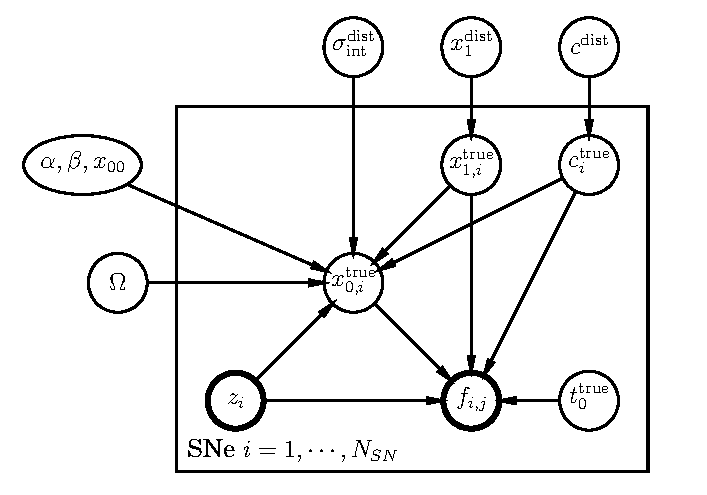
\includegraphics{images/snpgm}
%\caption{The basic hierarchical SALT2 model for ensembles of type Ia supernovae.}
%\label{fig:model1}
%\end{figure}

\subsection{Observed Values}

There are three different quantities that are assumed to be observed values or
`data' in the Bayesian sense.
\begin{itemize}
\item The cosmological redshift $z_i$ of the $i^{\rm th}$ supernova.
\item The observed flux of the $i^{\rm th}$ supernova in the $j^{\rm th}$ epoch, denoted by $f_{i,j}$. (The bandpass and epoch of each observation are assumed known.)
\item The noise in each of the measurements of flux, which is due to noise in the number of photons from both the supernova-source and the sky background, and in the reference image used in the image differencing. In this model, we will assume that this is entirely due to the sky background, which is measured independently, and perfectly. We denote the RMS value of this single, Gaussian noise component by
$\sigma^{sky}_{i,j}$ where, as above, $i$ indexes the supernova and $j$ indexes the epoch of observation of the supernova.
\end{itemize}

\subsection{Model Parameters}

The SALT2 model can be summarized as follows:
\begin{itemize}

    \item We have a light curve model for the $i^{\rm th}$ supernova with parameters $\{t_0, x_0, x_1, c, z\}_i$, that provides the predicted flux values that enter into the sampling distribution (likelihood) for the flux values at different times:
    $P(f_{i,j} \vert \{t_0, x_0, x_1, c, z\}_i, \{\sigma_{i,j}\} )$.

    \item It is common to parameterize supernovae in terms of magnitudes rather than fluxes, writing,
    \be
    m_B^{\star} = -2.5 \log_{10}{(f_B^{\star})}, \quad f_B^{\star} = \int d\lambda T(\lambda) \frac{d S}{d\lambda}(\lambda, p=0).
    \ee
    $m_B^{\star}$ is related mostly to $x_0$, since the contribution from terms involving $c$ and $x_1$ to this quantity is constrained to be exactly $0$ by defining the SALT2 model to give $p=0$ at the central wavelength of the Bessell B band. In this very good approximation, $m_B^{\star} = -2.5 \log_{10}{(x_0)} - 2.5 \log_{10}{(F_0)},$ where $F_0$ is a constant which can be evaluated. Thus, we will treat $x_0$ and $m_B^{\star}$ as interchangeable quantities, and redefine for convenience:
    \be
    m_B^{\star} = - 2.5 \log_{10}{(x_0)} , \qquad M_i \rightarrow M_i + 2.5\log_{10}{(F_0)}
    \ee

    \item An individual model supernova is completely specified by the set of parameters $\thetalctrue = \{ t_0, m_B^{\star}, x_1, c, z\}$: these are the parameters that can be inferred from the lightcurve data for a single supernova. Equivalently, to predict the observed fluxes for one supernova, we only need to specify the parameters in $\thetalctrue$. Some may prefer to work entirely in flux units, with $\thetalctrue = \{ t_0, x_0, x_1, c, z\}$.

    \item When considering an ensemble, we make a Tripp ansatz that relates the peak absolute magnitude $M_{B}$ in the rest frame Bessell B band to the stretch and color parameters ${x_1, c}$ and a standard candle absolute magnitude $M_i$:
    \be
    M_{B,i} = M_i + \beta c_i - \alpha x_{1,i},
    \ee
    so that the peak magnitude $m_B^{\star}$ in Bessell B band calculated from
    the model is related to the distance modulus $\mu(z,\Omega)$ by
    \bea
      m_{B,i}^{\star} &=& \mu_i + M_{B,i} \\
                      &=& \mu_i + M_i + \beta c_i - \alpha x_{1,i}.
    \eea
    In terms of probability distributions, we can write
    $P(m_{B}^{\star} \vert z,\Omega,M,\beta,c,\alpha,x_1) = \delta(m_{B}^{\star} - \mu - M - \beta c + \alpha x_1)$.

\end{itemize}


\subsection{Conditional PDFs}

We model the intrinsic dispersion of supernova properties as follows:
\begin{itemize}

    \item It is well known that standardization as described above is not complete, and that the distance moduli derived using the above equations have residual scatter. There is some evidence that this scatter is different in different bands, and therefore cannot be completely modelled by a scatter in $M_i$ above, but we shall ignore this for now and model this by assuming that \be M_i \sim \mathcal{N}(\bar{M}, \sigma_{\rm int}), \ee where $\sigma_{\rm int}$ is the intrinsic dispersion hyper-parameter which we aim to infer.

    \item Likewise, the stretch and color parameters $x_1$ and $c$ are taken to be similarly simply distributed, with
    \bea
       x_{1,i} &\sim& \mathcal{N}(\bar{x_1}, \sigma_{x_1}), \\
       c_i     &\sim& \mathcal{N}(\bar{c}, \sigma_{c}).
    \eea

    \item The distribution of peak times $t_0$ is taken to be uniform over the survey window, with no hyper-parameters to be inferred.

\end{itemize}


\subsection{Hyper-parameters}

At the top level of inference we have the following hyper-parameters, on top of the ones that parametrize the conditional PDF for the SN properties:

\begin{itemize}

\item $\alpha$ and $\beta$. These are gradient-like parameters, for which a prior PDF something like $1/(1+\theta^2)$ might be appropriate.

\item Cosmological parameters $\Omega$, with the usual priors.

\end{itemize}


\subsection{Probabilistic Graphical Model}

% Phil is here. Thinking maybe the next step should be to
% make a PGM that corresponds to the above model, for discussion with Josh.



\subsection{Rahul's Further Derivations}

Combining these, we can obtain the probability distributions
$ P(m_B^{\star}\vert \Omega, M_0, z, x_1, c)$ or equivalently $P(x_0 \vert \Omega, M_0, \sigma_{int}, x_1, c, z)$:
\beqn
P(m_B^{\star} \vert \Omega, M_0, z, x_1, c, \sigma_{int} ) &=&
\int dM P(m_B^{\star} \vert M, \Omega, \alpha, \beta, x_1, c)P(M \vert M_0, \sigma_{int}) \\
&=&
\mathcal{N}(\mu(\Omega, z) - \alpha x_1 + \beta c + M_0, \sigma_{int}^2)
\eeqn

While, we are assuming that
\be
P(x_1 , c \vert \Omega, M_0, z, \sigma_{int}) = P(x_1, c) = P(x_1) P(c)
\ee
which we may relax in other models. In this model,  we have
\beqn
P(\thetalctrue \vert \Omega, \alpha, \beta, z, M_0, \sigma_{int}) &\equiv& P(m_B^{\star} \vert x_1, c, t_0, \Omega, z, \alpha, \beta, M_0, \sigma_{int}) \nonumber \\
&\times& P(x_1, c, t_0, z, \Omega, \alpha, \beta, M_0, \sigma_{int})\\
&=& P(m_B^{\star} \vert x_1, c, M_0, \sigma_{int}, \Omega, z, \alpha, \beta) \\
&\times& P(x_1, c, t_0 ,\sigma_{int}) P(\Omega, z, \alpha, \beta) \nonumber\\
&=& \mathcal{N}(\mu(\Omega, z) - \alpha x_1 + \beta c + M_0, \sigma^{int}) \\
&\times&  P(x_1, c, t_0 ,\sigma_{int}) P(\Omega, z, \alpha, \beta)
\eeqn



\subsection{Posterior Samples of the Cosmology}
The quantity we are interested in is the posterior distribution of the cosmological parameters $\Omega$ (where we will use $\Omega$ to denote the set of
cosmological parameters, given the set of measurements $f_{i, j}$ , $\sigma_{i,j}$ which is
\be
P(\Omega \vert \{f_{i,j}, \sigma_{i,j}, z_i,  \}) =
        \int d\alpha d\beta d\sigma_{int}d M_0 P(\Omega, \alpha, \beta, M_0, \sigma_{int} \vert \{f_{i,j}, \sigma_{i,j}, z_i\})
\ee
We would like to do this integral by drawing samples from the space of cosmological parameters $\Omega, \alpha, \beta, M_0, \sigma_{int}$ with their frequencies
according to above probability distribution. This requires evaluating
$
P(\Omega, \alpha, \beta, M_0, \sigma_{int} \vert \{ f_{i,j}, \sigma_{i,j}, z_i\})
,$ at least, upto a constant of proportionality. We try to evaluate this using
samples of individual light curve parameters inferred without any prior on
cosmology.
\be
P(\Omega, \alpha, \beta, \sigma_{int}, M_0 \vert \{ f_{i,j}, \sigma_{i,j}, z_i\})
    \propto P(\{ f_{i,j}\} \vert \Omega, \alpha, \beta, M_0, \sigma_{int}, \{\sigma_{i,j}, z_i \} ) P(\Omega, \alpha, \beta, M_0, \sigma_{int})
\ee
To get the RHS, we need
\beqn
 P(\{f_{i,j}\} \vert \Omega, \alpha, \beta, \sigma_{int}, M_0, \{\sigma_{i,j},z_{i}\}) &=& \int  \prod_{i} d\thetalctrue_{i} P(\{f_{i,j} \}, \vert \{\sigma_{i,j}, \thetalctrue_i, z_i \}) \\
  &\times& P(\{\thetalctrue_i \}\vert \Omega, \alpha, \beta, \sigma_{int}, M_0, z_i) \nonumber\\
 &=& \prod_i \int d\thetalctrue_i  P(\{f_{i,j} \}, \vert \{\sigma_{i,j} , z_i, \thetalctrue_i, z_i \})\\
 %P(\{\thetalctrue_i \}\vert \Omega, \alpha, \beta, z_i)
 &\times& P({t_0}_i)  P({x_1}_i) P(c_i)  \mathcal{N}(\mu(\Omega, z) - \alpha {x_1}_i + \beta c_i + M_0, \sigma^{int})  \\
 &=& \prod_i \left( \int d\thetalctrue_i \Phi_i (\thetalctrue_i) w_i (\thetalctrue_i)\right) \\
 &=& \prod_i I_i
\eeqn
where  $\Phi_i(\thetalctrue_i)$ is proportional to the posterior distribution of the model parameters $\thetalctrue_i$ of i'th supernova
\be
\Phi_i(\thetalctrue_i) \equiv P(\{f_{i,j} \}, \vert \{\sigma_{i,j} , z_i, \thetalctrue_i, z_i \})P(t_{0})P(x_1)P(m_B^{\star})P(c)
\ee
and therefore $w_i(\thetalctrue_i)$ are given by
\be
w_i = \mathcal{N}(\mu(\Omega, z) - \alpha {x_1}_i + \beta c_i + M_0, \sigma^{int}) / P(m_B^{\star})
\ee
Using the equal weight samples (indexed by $j$) of posteriors of light curve model parameters obtained from the individual light curves, we can do the individual integrals $I_i$ for each
supernova
\be
I_i \approx \frac{1}{N_i} \sum_j \thetalctrue_{i,j} w_i ( \thetalctrue_{i,j})
\ee
where $N_i$ is the number of samples of light curve model parameters of the
$j'\rm{th}$ supernova.
The first term is the posterior distribution of the light curves parameters
found separately in a previous stage. The integral in the last equation for each SN is then a sum over samples indexed by $j$

\end{document}
